\documentclass[prb,preprint]{revtex4-1} 

\usepackage{amsmath}  
\usepackage{amsfonts} 
\usepackage{graphicx} 
\usepackage{gensymb}

\begin{document}

\title{Measurement of Faraday Rotation and Calculation of the Verdet Constant for a Glass? Rod}

\author{Frances Yang}
\email{fyang@smith.edu} 

\author{Isabel Lipartito}
\email{iliparti@smith.edu}
\affiliation{Department of Physics, Smith College, Northampton, MA 01063}

\date{\today}

\begin{abstract}
{We aim to calculate the Verdet constant relating the change in magnetic field through a medium sample to the change in polarization angle of light traveling through the medium.  A $650\ nm$ laser was sent through a solenoid containing a {\bf glass?} rod and an adjustable polarizer and detected by a photodiode. A lock-in amplifier was used on the voltage output of the photodiode to reduce background noise. The phase offset was found by performing a non-linear least squares regression on the output voltage ($V$) versus polarizer angle ($\theta$) data for four $B$ fields. The Verdet constant for the sample was calculated from phase differences due to changes in the magnetic fields and found to be $15.1 \pm 1.2 \ (T\cdot m)^{-1}$. Other value  $19.88 \pm 0.11 \ (T\cdot m)^{-1}$}
\end{abstract}

\maketitle 
\section{Aims}
{a.  To demonstrate the Faraday effect of the rotation of the plane of polarization of light as it travels through magnetic fields of different magnitudes.

b.  To calculate the Verdet constant relating the change in polarization angle to the change in magnetic field.}
\begin{equation}
\Delta \phi =V_{c} \Delta B L{_{sample}}
\end{equation}

\section{Introduction} 

{The Faraday Effect is a magneto-optical phenomenon in which light of a single wavelength, traveling through certain materials subject to a magnetic field, experiences a shift in the plane of polarization. These materials, called birefringent, have different refractive indices for the right and left circular polarizations of light. This changes the relative phase angle between the two polarizations as the light travels through, thus rotating the overall polarization plane.

As shown in Equation 1, the Verdet Constant ($V_{c}$) relates the change in magnetic field of a medium to the change in polarization angle of the traveling light.  $V_{c}$ is specific to any medium.  There are two ways in which we can calculate $V_{c}$.  By Malus's Law, $I(\theta)$=$I_{0}*\cos^{2}(\theta)$, where $I$ is the intensity of measured light through a polarization filter of angle $\theta$ with respect to the maximal polarization angle.  Similarly, for voltage output, $V(\theta)$=$V_{0}*\cos^{2}(\theta)$.  Once we add into this set-up a magnetic field through which the light can travel, we will observe the voltage output equation to have a phase shift, $\theta$:  $V(\theta)$=$V_{0}*\cos^{2}(\theta+\phi)$.

One way to calculate $V_{c}$ is to measure the phase shift, $\phi$ for multiple magnetic fields:  collecting data for $V(\theta)$ for a full 0-360 degree range of $\theta$ and comparing data for different magnetic fields to a base data set of the same set up, where there is no magnetic field.  $\theta$ can be plotted against $B$- they should have a linear relationship- and by finding the slope of that linear fit, $\frac{\partial \theta}{\partial B}$ will be found and thus $V_{c}$ by Equation 1.}

{Another way to find $V_{c}$ is to notice that $\frac{\partial \theta}{\partial B}= \frac{\partial \theta}{\partial V}*\frac{\partial V}{\partial B}$}

\section{Procedure}
{Polarized light came from a $650\ nm$ laser, driven by a 400 $kHZ$ square wave from a function generator. A 10 layer, with 140 turns/layer solenoid with a DC resistance of $1.6\ \Omega$ provided a magnetic field that could be varied by changing the current passing through the solenoid.  We measured the magnetic field at the center of our solenoid to be $10.6\ mT/A \pm .05\ mT.$ Our sample, a {\bf glass rod}, was centered inside the solenoid. The light is passed through a polarizer and detected by a photodiode. }


\section{Results}
\begin{figure}
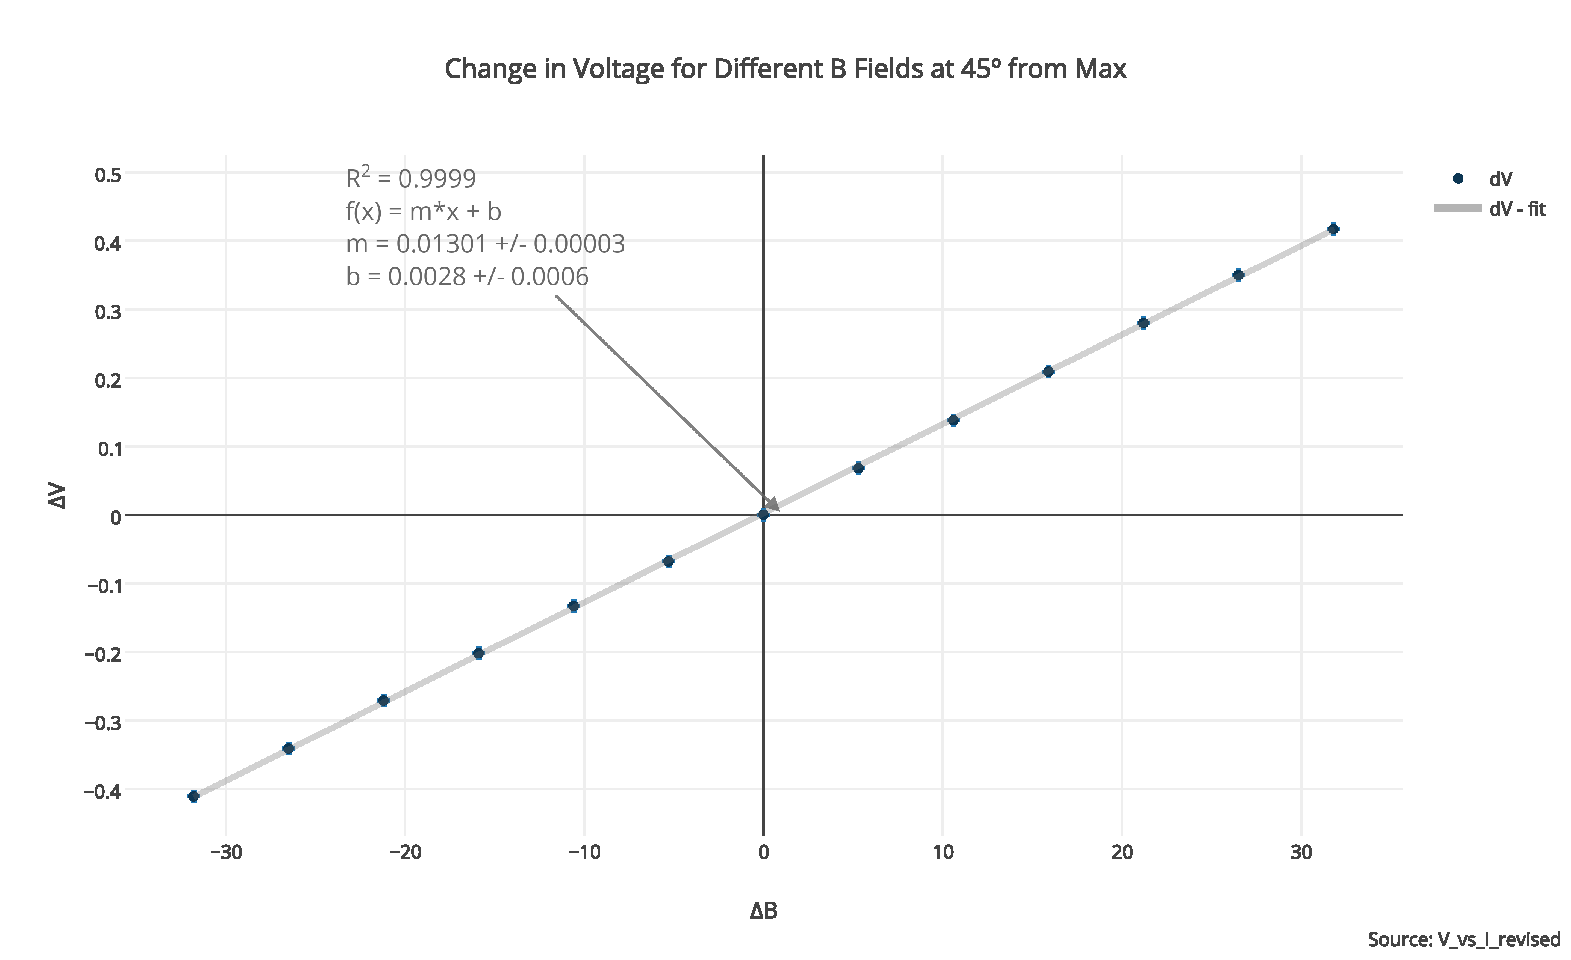
\includegraphics[width =6.5in]{change_in_voltage_for_different_b_fields_at_45_from_max.pdf}
\caption{\label{method2pic} The measured change in photodiode voltage for a change in the magnetic field at a polarizer angle 45\degree\  from the maximum voltage output. A linear fit was used to determine $\Delta V/\Delta B$.}
\end{figure}
\section{Analysis}


\section{Discussion}




\section{Conclusion}


\section{References}

\end{document}